\begin{frame}[fragile]{Manipulation de fichiers et répertoire : interface du mini-shell}
    \begin{itemize}[leftmargin=-12pt]
    \item<1->Première version de l'AST des commandes :
        \todo{reorganiser dans l'ordre le plus pertinent en fonction de la suite}
        \begin{lstlisting}[breaklines=false]
            type command =
                | Mkdir of string * int option (* mkdir dir []-m int] *)
                | Rm of string * bool          (* rm filename [-r] *)  
                | Ln of string * string * bool (* ln source dest [-s] *)
                | Ls of string option          (* ls [filename] *)
                | Cat of string list           (* cat files *)
        \end{lstlisting}
        
    \item<2-> Parser, et interpréteur de commandes :
         \begin{lstlisting}
            val parse : string -> command
            val exec_command : command -> unit 
        \end{lstlisting}
    \end{itemize}
\end{frame}  

\begin{frame}[fragile]{Parseur et interpréteur}

    \begin{itemize}[label=\small\ding{114}]
    \item<1-> Parseur : plusieurs solutions (\texttt{Args}, \texttt{Angstrom} etc..)
    \item<2-> Interpréteur : 
      \begin{lstlisting}
            let exec_command cmd = 
                match cmd with
                | Cat filename              -> failwith "todo"
                | Ln (source, dest, symb)   -> failwith "todo"
                | Mkdir (dirname, perm_opt) -> failwith "todo"
                | Rm (filename, recursive)  -> failwith "todo"
                | Ls name_opt               -> failwith "todo"
        \end{lstlisting}
    \end{itemize}
\end{frame} 

\begin{frame}{Implémentation de cat}

    \texttt{cat files} : concatène le contenu des fichiers \texttt{files} et les écrit dans la sortie standard.
    
    \subtt{Exemple}
    
    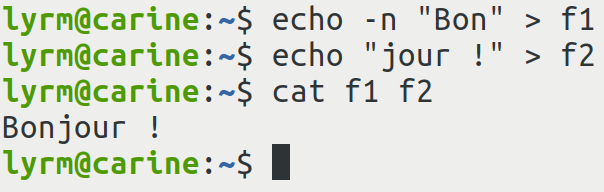
\includegraphics[width=0.5\textwidth]{slides/images/shell_cat.png}
    
    \pause\subtt{Pseudo-code}

    Pour chaque fichier de \texttt{files} : 
    \begin{itemize}[label=\small\ding{114}]
        \item ouvrir le fichier
        \item le lire et l'écrire sur la sortie standard = le copier sur stdout
        \item fermer le fichier
    \end{itemize}
\end{frame}

\begin{frame}[fragile]{\texttt{Unix} : lecture et écriture de fichiers}
    \begin{lstlisting}
        type file_descr         (* descripteurs de fichiers *)
        val stdin : file_descr  (* entree standard *)
        val stdout : file_descr (* sortie standard *)
        val stderr : file_descr (* sortie d'erreur standard *)
        
        type open_flag = (* modes d'ouverture *)
            | O_RDONLY 
            | O_WRONLY 
            | O_RDWR 
         (* |.. *)
        type file_perm = int (* droits (Ex : 0o777) *)
        
        val openfile : 
            string -> open_flag list -> file_perm -> file_descr
        val close : file_descr -> unit
        val read : file_descr -> bytes -> int -> int -> int
        val write : file_descr -> bytes -> int -> int -> int
    \end{lstlisting}
\end{frame}

\begin{frame}[fragile]{Implémentation de cat}
    \begin{itemize}[leftmargin=-10pt]
        \item<1->
            \begin{lstlisting}
                let exec_cat files = 
                    List.iter (fun file ->
                        let fd_in = 
                            Unix.openfile file [ Unix.O_RDONLY ] 0 in
                        copy_file fd_in fd_out;
                        Unix.close fd_in)
                    files
        \end{lstlisting}
        \item<2->
            \begin{lstlisting}
                let copy_file_stdout fd_in =
                  let buffer_size = 8192 in
                  let buffer = Bytes.create buffer_size in
                  let rec copy_loop () =
                    match Unix.read fd_in buffer 0 buffer_size with
                    | 0 -> ()
                    | r -> ignore (Unix.write stdout buffer 0 r);
                           copy_loop () in
                  copy_loop ()
            \end{lstlisting}
     \end{itemize}
\end{frame}


\begin{frame}[fragile]{\texttt{mkdir}, \texttt{rm -r} et \texttt{ls} : opération sur les répertoires}
      \begin{lstlisting}
          type file_perm = int (* ex : 0o777 *)
          val mkdir : string -> file_perm -> unit
          val rmdir : string -> unit
          
          type dir_handle
          val opendir : string ->  dir_handle
          val readdir : dir_handle -> string 
          val closedir : dir_handle -> unit
          
          (* Pour plus tard *)
          val chdir : string -> unit 
          val getcwd : unit -> string
          val chroot : string -> unit
    \end{lstlisting}
\end{frame}

\begin{frame}{Implémentation de mkdir}
    
\end{frame}

\begin{frame}{Implémentation de ls}

- Opendir, readdir, stat

inodes
    
\end{frame}

\begin{frame}[fragile]{AST évolué}
    \begin{itemize}[leftmargin=-10pt] 
         \item
        \begin{lstlisting}
            type cmd_kind =
                | Internal of command (* les commandes precedentes *)
                | External of string list (* la triche avec execv *)
                | Cd of string (* getcwd / chdir *)
            type redirection =
                | In of string (* > *)
                | Out of string (* < *)
            type command = cmd_kind * redirection list
            type t = 
                | Command of command
                | Pipe of t * t (* | *)
                | And of t * t (* exit status *)
                | Or of t * t
            val execute : t -> unit
        \end{lstlisting}
    \end{itemize}

\end{frame}

\begin{frame}{Répertoire courant}

\end{frame}


\begin{frame}{Gestion des erreurs}

\end{frame}

\begin{frame}{Processus}

Recap sur les processus: scheduling pré-emptif dans Linux

Liste de processus: toutes les 10ms on execute l'un des processus.
Structure de donnée en mémoire pour sauvegarder l'état d'un processus.

État d'un processus: 
- état des registres processeur
- file descriptors
- répertoire courant
- variables d'environnement

\end{frame}
